\documentclass[a4paper]{article}
\usepackage[utf8]{inputenc}
\usepackage[T1]{fontenc}
\usepackage[slovene]{babel}
\usepackage{lmodern} 

\usepackage{amsmath}  
\usepackage{amsthm}  
\usepackage{amssymb} 
\usepackage{graphicx}
\usepackage{float}

\title{\textit{Problem največjega pretoka}}
\author{Žan Kastelic, Lara Vidmar}
\date{~december 2020}

\begin{document}
\begin{titlepage}
 \maketitle

\end{titlepage}

\section{Opis problema}
Pri problemu največjega pretoka imamo pretočno omrežje, po katerem teče tekočina. Omrežje vsebuje dve oblikovani vozlišči, $s$ in $t$. Iščemo največji možen pretok med njima. Vozlišče $s$ se imenuje \textbf{izvor} in nima nobene vstopne povezave. Vozlišče $t$ pa \textbf{ponor} in nima nobene izstopne povezave.

PODATKI: 
\begin{itemize}
\item Imamo usmerjen graf $G = (V, E)$ z v naprej oblikovanima vozliščema $s $ in $t.$ Pri tem je $V$ množica vozlišč in $E$ množica povezav v grafu.
\item Na vsaki povezavi $(v_i, v_j) \in E$ imamo nenegativno realno število $c_{ij}$ tj. prepustnost ali kapaciteta povezave $(v_i, v_j).$ Prepustnost $c_{ij}$ lahko razširimo na vse pare vozlišč:  $c(i, j) = \begin{cases} c_{ij}, & \mbox{če }(v_i, v_j)\mbox{$ \in$ E} \\ 0, & \mbox{če }(v_i, v_j)\mbox{ $\not\in$ E} \end{cases}$
\item Urejeno četvorko (G, s, t, c) imenujemo \textbf{pretočno omrežje.}
\end{itemize}

Pri zgornjih podatkih iščemo največji pretok, ki je preslikava $f: V \times V \rightarrow \mathbb{R}.$ $f(i,j) < 0$, pomeni tok $|f(i,j)|$ od j proti i. Pri tem mora bit zadoščeno naslednjim pogojem. 
\begin{itemize}
\item \textit{Ustreznost pretoka}:  $f(i, j) \le c(i, j) $ za $\forall i, j \in V$
\item \textit{Antisimetričnost pretoka}: $f(i, j) = - f(i, j)$ za vse $i, j \in V$
\item \textit{Kirchhoffovi zakoni}: $\sum i \in V f(i, j) = 0 $ za vse $j \in V \setminus  \left \{ s, t \right \}$ 
\end{itemize}
Velja $f(i, j) = - f(i,j) = 0. $
Če je $f$ pretok, je povezava $(v_i, v_j) \in E$ \textbf{zasičena,} če velja $f(i,j) = c(i,j).$ Oziramo \textbf{nenasičena}, če je $f(i,j) < c(i,j).$ 

\textbf{Velikost pretoka f} je $$|f|= \sum_{i \in V} f(i,t). $$


\section{Načrt dela}

Najinega projekta se bova lotila v programu R. Najprej bova implementirala algoritem za iskanje največjega pretoka v acikličnem povezanem grafu. Pomagala si  bova z Edmonds-Karp algoritmom. Algoritem najprej poišče poti od izvora s do ponora t, z uporabo iskanja v širino, potem pa s  Ford-Falkersonovega algoritmom poišče največji pretok. Midva bova napisala algoritem, ki bo prvo izpisal vse poti, potem pa bova gledala minimum prepustnosti določene poti. Kot sva ugotovila obstaja v programu R že vgrajena funkcija za iskanje največjega pretoka tj. maxFlowFordFulkerson. Poiskušala bova primerjat algoritma in ugotoviti kateri je bolj učinkovit. 

Grafe bova implementirala s pomočjo matrike sosednosti, kjer bodo prepustnosti izbrane naključno iz že v naprej podanega intervala celih števil. Če utež ne bo enaka 0, potem bo ta povezava obstajala. Za lažjo predstavo bo funkcija graf tudi narisala. 

Kot drugo bova poizkušala graf implementirati s pomočjo naključnih geometrijskih grafov. Neka povezava bo obstajala, če bo njena povezava manjša ali enaka od nekega števila r. Tem povezavam bova določila smer in nato še naključne uteži.

Eksperimente bova delala na zgoraj definiranih grafih, ki jim bova odstranila eno ali več vozlišč, odstranila povezave, zamenjala smer povezave. Opazovala bova kako se pretok spreminja in poizkušala iz tega dobiti kakšno lastnost oz. bova opisala opažanja. 

\section{Opis programa}

Najprej sva generirala matriko, v kateri so generirani podatki grafa. Pri tem so elementi matrike uteži, ki so naključne. Kombinacija vrstice in stolpca pa predstavlja povezavo (na primer (vrstica 4, stolpec 6) pomeni povezava iz oglišča 4 v 6). Ker pri iskanju pretoka potrebujeva acikličen graf, so v matriki v prvem stolpcu, v zadnji vrstici in na diagonali same ničle. Iz nje sva potem generirala graf. Da bi lahko napisala funkcijo, ki bo iskala največji pretok, sva potrebovala tabelo, v kateri bodo v prvem stolpcu vstopna vozlišča povezave, v drugem izstopna vozlišča povezave, v tretjem pa uteži. To sva naredila v funkciji $\text{oceti\_in\_sinovi}$. Najvecji pretok sva poiskala tako, da sva locirala pot od izvora (vozlišče 1) do ponora (vozlišče z največjo številko) in skoz njo spustila največi možen pretok. Potem sva matriko posodobila, tako da sva ostranila povezave z ničelno utežjo in postopek ponovila. Kot sva ugotovila, je ta algoritem delal zelo počasi in je izračunal pretok za grafe do 7 vozlišč. 

Zato sva generirala nov algoritem za iskanje pretoka, pri tem sva si pomagala psevdokodo Edmonds-Karp algoritma, kot je prikazana na sliki \ref{fig1}. 


\begin{figure}[H]
\centerline{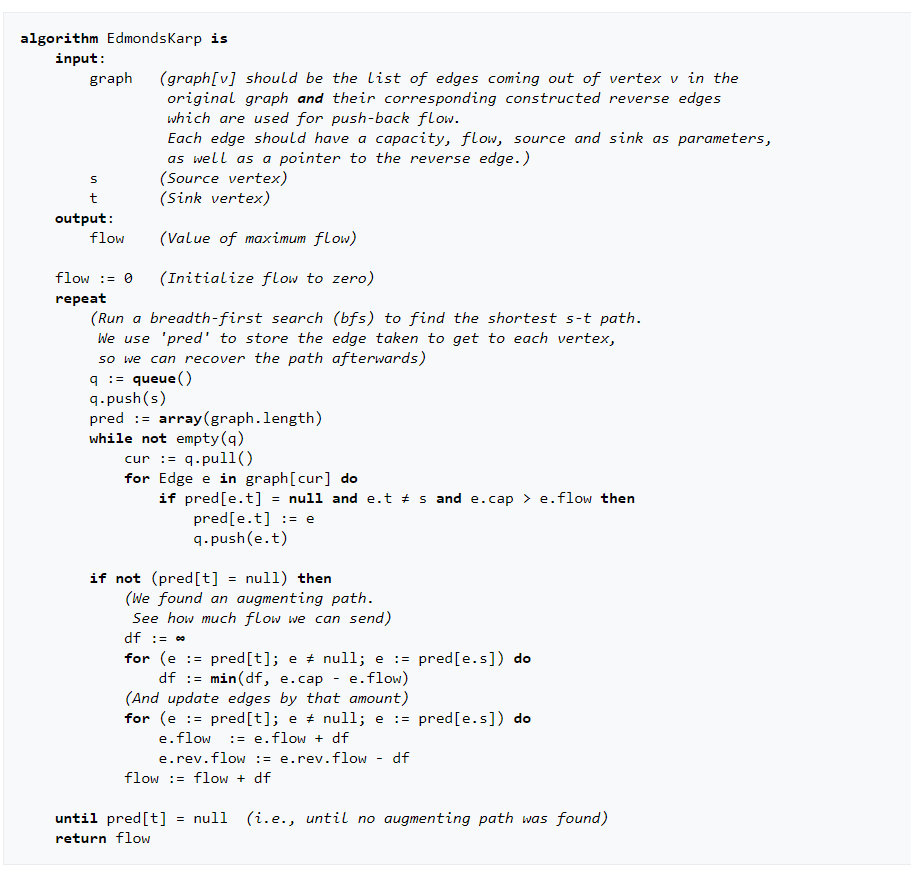
\includegraphics[scale=.5]{edmondkarp.PNG}}
\caption{Psevdokoda Edmonds-Karp algoritma.}
\label{fig1}
\end{figure}

Najprej sva spremenila najino matriko v igraph, kateri je veliko bolj učinkovit. Napisala sva algoritem $\text{pregled\_v\_sirino}$, ki išče poti od izvora do ponora. S pomočjo tega pa sva napisala $\text{edmonds\_karp}$ algoritem. Pri tem sva za odstranjevanje povezav in lociranje minimalnih utezi uporabljala vgrajene funkcije od igrapha. 

Kot sva že napovedala v načrtu dela, sva generirala geometrijske grafe. Razdelila sva jih na tri tipe in sicer, geometrijski grafi, ki imajo za uteži kar razdalje med točkami, potem grafe, ki imajo za uteži inverz razdalj in še zadnje, ki imajo naključne uteži.  Pri tem sva morala bit previdna, da je točka, ki je najbližje izhodišču markirana z 1, tista najdlje oddaljena pa je označena s številom točk. Velikost grafa je odvisna od števila $r$, ki predstavlja razdaljo med točkami. Večji kot je $r$ več povezav bo v grafu. 


\section{Generiranje podatkov}
Podatke sva najprej generirala za navadne grafe, ki sva jih pridobila iz matrike, potem pa še za geometrijske grafe. Pogledala sva kako se pretok spreminja, če odstranimo povezavo, ki ima minimalno utež in kako, če odstranimo povezavo z maksimalno utežjo. Potem pa še, kako se spremeninja pretok, če odstraniva naključno točko, ki ni izvor oziroma ponor. Funkcije sva generirala tako, da nama vrne tabelo, ki prikazuje pretok, kjer so  vrstice vrednosti za različno število točk, v stolpcih pa koliko povezav oz. koliko točk sva odstranila. Pri navadnih grafih sva gledala, kaj se dogaja s pretokom, če so vse uteži enake. Le pri tem sva ugotovila nek algoritem, katerega sva tudi napisala. 

Pri geometrijskih grafih sva funkcije generirala na podoben način. Pri funkcijah, ki odstranjujejo povezave in točke, sva vse vrste geometrijskih grafov združila v eno funkcijo. In sicer tako, da sva v argument dodala tudi $tip$, kateri predstavlja vrsto geometrijskega grafa, tj. $\text{igraf\_razdalje\_so\_utezi}$ pri tem napišemo $tip = 1$, $\text{igraf\_razdalje\_so\_inverz}$ je $tip = 2$ in še $\text{igraf\_utezi\_so\_nakljucne}$, ki je $tip = 3.$

Ker so geometrijski grafi zelo odvisni od razdalje $r$, naju je zanimalo tudi kako se spreminja pretok, če spreminjava $r$. 

\section{Opis in razlaga eksperimentov}

Eksperimente sva delala na grafih z 10 točkami in gledala njihov pretok. Podatke bova predstavila v grafih, saj so tako najbolj razvidne spremembe. Ker večina grafov generirava naključno, je pretok veliko odvisen tudi od naklučja uteži in povezav. 

\pagebreak
\subsection{Grafi generirani s pomočjo matrike.}

$\bullet $  Na grafu \ref{fig2} je razvidno, da pri grafih, kjer imajo vse povezave iste uteži, se pretok povečuje linearno s večanjem uteži in večanjem število točk. 
\begin{figure}[H]
\centerline{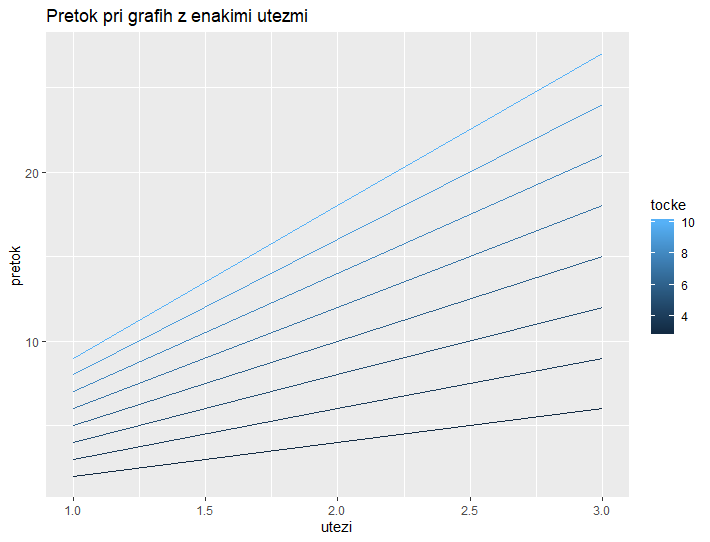
\includegraphics[scale=.5]{p1.PNG}}
\caption{Pretok na grafih z enakimi utežmi.}
\label{fig2}
\end{figure}


$\bullet $ Na grafu \ref{fig3} je prikazano spreminjanja pretoka, če grafu odstranjujemo povezavo z minimalno utežjo. Kot pričakovano je pretok vsakič manjši.  

\begin{figure}[H]
\centerline{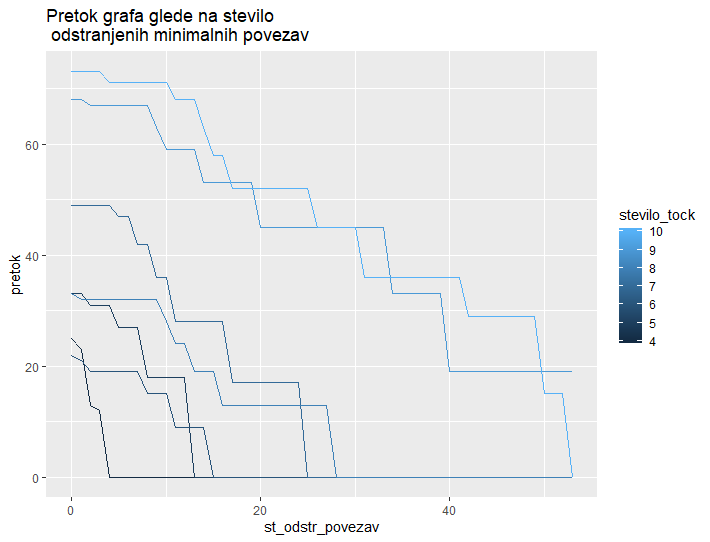
\includegraphics[scale=.5]{p3.PNG}}
\caption{Pretok na grafih z naključnimi utežmi, odstranimo povezavo z min. utežjo. }
\label{fig3}
\end{figure}

\pagebreak
$\bullet $ Na grafu \ref{fig4} je prikazano kako se pretok spreminja, če grafu odstranjujemo povezavo z največjo utežjo. Graf je podoben zgornjemu, le da se pri tem pretok veliko hitreje manjša v primerjavi z zgornjim grafom. 
\begin{figure}[H]
\centerline{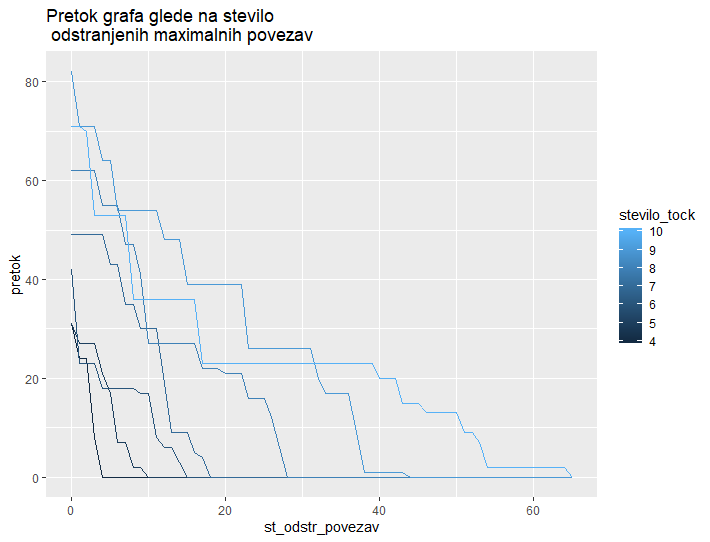
\includegraphics[scale=.5]{p4.PNG}}
\caption{Pretok na grafih z naključnimi utežmi, odstranimo povezavo z max. utežjo. }
\label{fig4}
\end{figure}

$\bullet $ Na grafu \ref{fig5} je prikazano spreminjanja pretoka, če odtranjujemo točke. Vsak korak odtstranimo eno točko več. Ta graf je veliko bolj linearen od zgornjih dveh, saj z odstranitvijo ene točke,lahko odstranimo veliko več kot samo eno povezavo. 
\begin{figure}[H]
\centerline{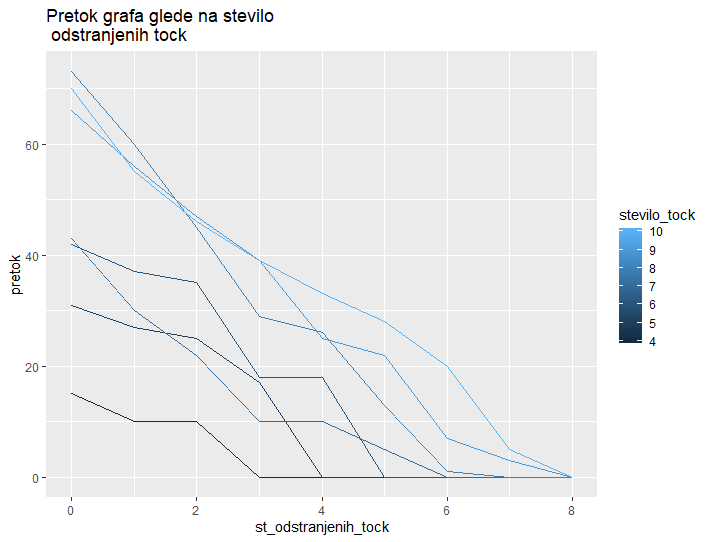
\includegraphics[scale=.5]{p5.PNG}}
\caption{Pretok na grafih z naključnimi utežmi, odstranimo naključne točke.}
\label{fig5}
\end{figure}

\subsection{Geometrijski grafi}
Sledijo podatki za geometrijske grafe. Ločeni so glede na tipe utezi. \\

$\rightarrow $ Geometrijski grafi, ki jim odstranjujemo točke. \\

$\ast$ Na grafu \ref{fig6} je prikazan geometrijski graf, ki ima za uteži kar razdaljo med točkami. Kot vidimo pretok linearno pada. Vsakič ko odstranimo po eno točko več je pretok seveda manjši.

\begin{figure}[H]
\centerline{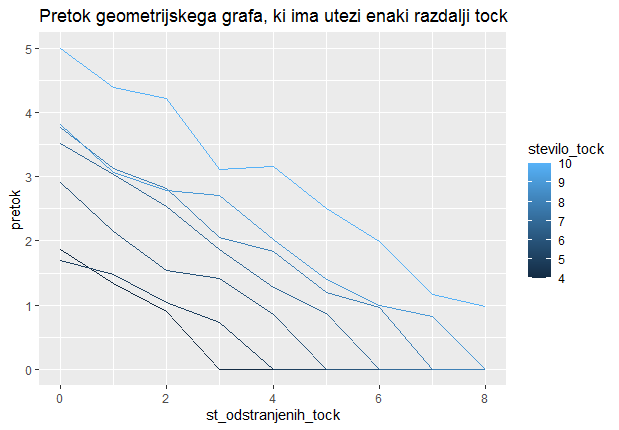
\includegraphics[scale=.5]{p6_1.PNG}}
\caption{Pretok pri geometrijskem grafu ($tip = 1$), ki mu odstranjujemo točke.}
\label{fig6}
\end{figure}

$\ast$  Na grafu \ref{fig7} je prikazan geometrijski graf, ki ima uteži inverz razdalj med točkami. Kar pomeni točki, ki sta bližje skupaj bosta imeli večjo utež, kot pa tisti, ki sta bolj oddaljeni. Če graf pogledamo brez nenadnih skokov v pretoku, kateri nastanek bova objasnila kasneje, je nekako podoben prejšnjemu. Le da je pri tem pretok veliko večji že od začetka. 

\begin{figure}[H]
\centerline{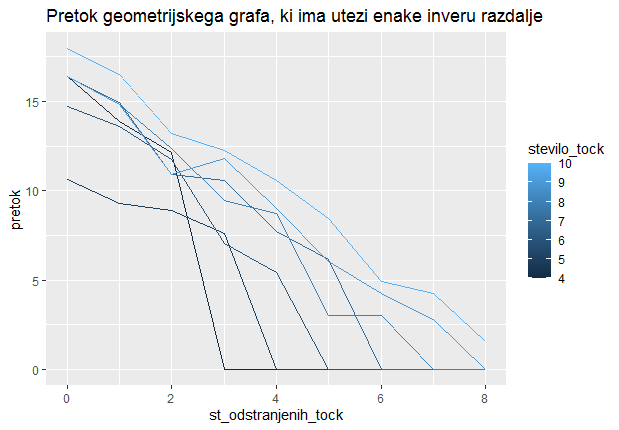
\includegraphics[scale=.5]{p6_2.PNG}}
\caption{Pretok pri geometrijskem grafu ($tip = 2$), ki mu odstranjujemo točke.}
\label{fig7}
\end{figure}

$\ast$  Na grafu \ref{fig8} je prikazan geometrijski graf, ki ima za uteži naključna cela števila do 10. Pri tem, poleg veliko večjega začetnega pretok, ki je posledica večjih uteži, ne opazimo razlike od zgornjih dveh. Pretok se z vsako odstranjeno točko manjša.

\begin{figure}[H]
\centerline{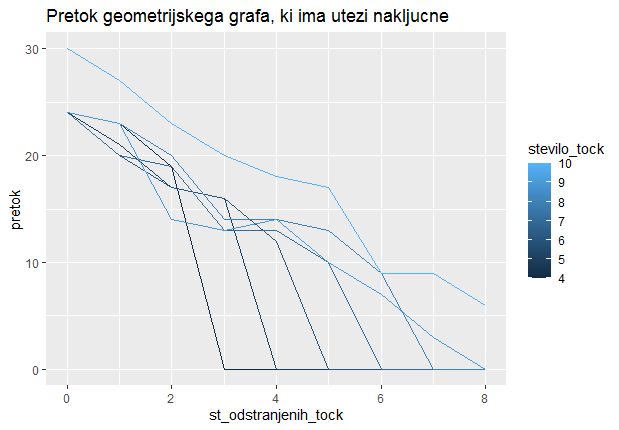
\includegraphics[scale=.5]{p6_3.PNG}}
\caption{Pretok pri geometrijskem grafu ($tip = 3$), ki mu odstranjujemo točke.}
\label{fig8}
\end{figure}

Lahko bi rekli, da je neglede na to kakšen geometrijski graf uzamemo, pretok padajoč glede na število odstranjenih točk. \\

$\rightarrow $  Geometrijski grafi, ki jim odstranimo minimalno utež na povezavi. \\

$\ast$ Na grafu \ref{fig9} je prikazan geometrijski graf, ki ima za uteži kar razdaljo med točkami. Odstranjujemo mu minimalno povezavo. Pretok je padajoč. Če povezava, ki je bila odstranjena ni bila na poti od izvora do ponora, bo seveda pretok ostal nespremenjen, zato je pri tem velikokrat ravna črta na določeni višini. Drugače pa se slej ko prej pretok približa ničli. 
\begin{figure}[H]
\centerline{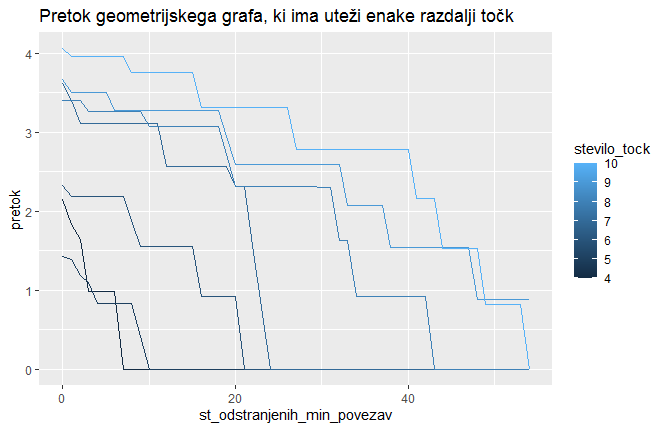
\includegraphics[scale=.5]{p8.PNG}}
\caption{Pretok pri geometrijskem grafu ($tip = 1$), ki mu odstranjujemo minimalno utež na povezavi.}
\label{fig9}
\end{figure}

$\ast$ Na grafu \ref{fig10} je prikazan geometrijski graf, ki ima uteži inverz razdalj med točkami. Pri tem je zgodba podobna kot pri prejšnem, le da je tukaj pretok veliko večji, zaradi večjih uteži.
\begin{figure}[H]
\centerline{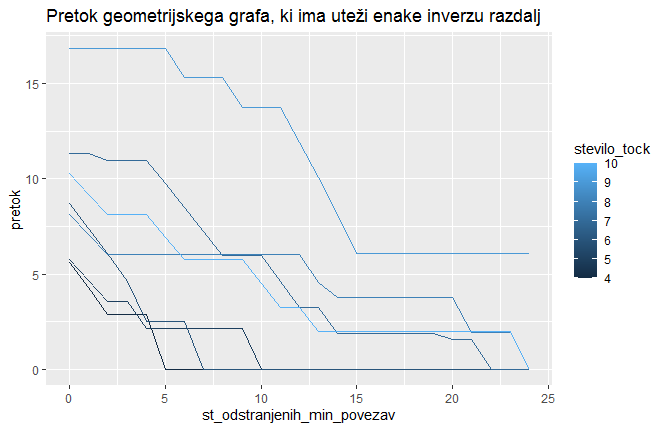
\includegraphics[scale=.5]{p7.PNG}}
\caption{Pretok pri geometrijskem grafu ($tip = 2$), ki mu odstranjujemo minimalno utež na povezavi.}
\label{fig10}
\end{figure}

$\ast$ Na grafu \ref{fig11} je prikazan geometrijski graf, ki ima za uteži naključna cela števila do 10. Tukaj je padanje veliko bolj konsistentno, to bi lahko pripisali bolj enakomerno razporejenim utežem v grafu. Saj ker generiramo graf z delimi števili do 10, je možnosti za različne uteži bolj malo. 
\begin{figure}[H]
\centerline{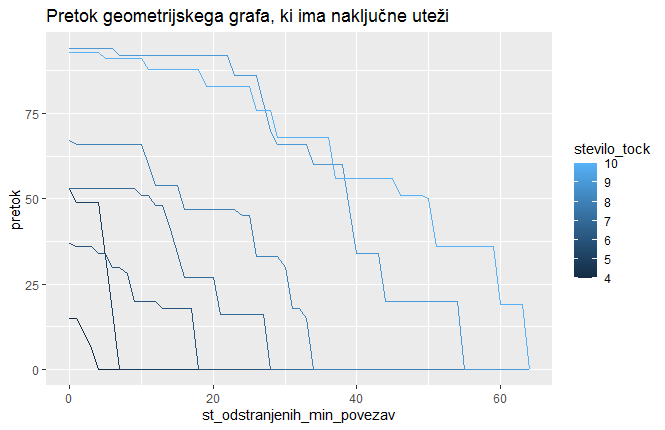
\includegraphics[scale=.5]{p9.PNG}}
\caption{Pretok pri geometrijskem grafu ($tip = 3$), ki mu odstranjujemo minimalno utež na povezavi.}
\label{fig11}
\end{figure} 

$\rightarrow $ Geometrijski grafi, ki jim odstranimo maksimalno utež na povezavi. \\

$\ast$ Na grafu \ref{fig12} je prikazan geometrijski graf, ki ima za uteži kar razdaljo med točkami. Ke odstranimo maksimalno utež se pretok veliko hitreje pride do 0. 
\begin{figure}[H]
\centerline{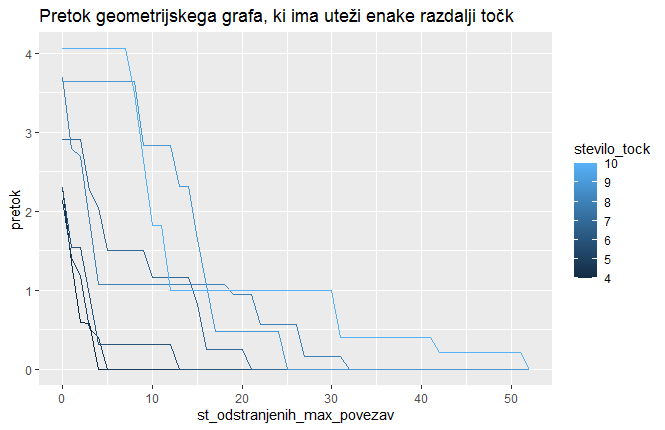
\includegraphics[scale=.5]{p8_1.PNG}}
\caption{Pretok pri geometrijskem grafu ($tip = 1$), ki mu odstranjujemo maksimalno utež na povezavi.}
\label{fig12}
\end{figure}

$\ast$Na grafu \ref{fig13} je prikazan geometrijski graf, ki ima uteži inverz razdalj med točkami. Enako situacijo imamo tudi tukaj, le da štartamo iz večjega pretoka. Je pa padanje nekoliko počasnejše. To bi lahko pripisali temu, da so inverzi razdalj večji, se pravi so uteži večje. %to nevem če je res 
\begin{figure}[H]
\centerline{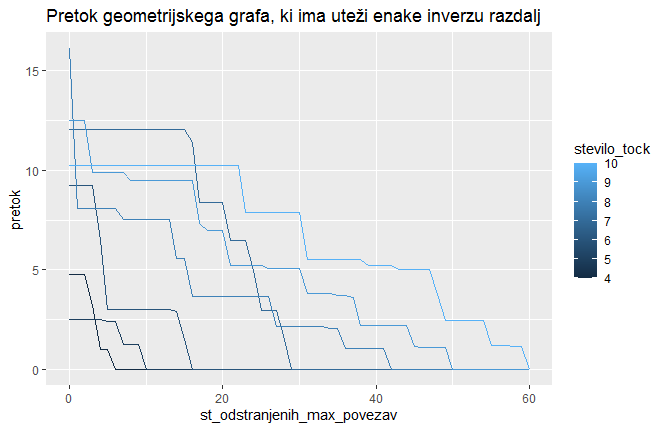
\includegraphics[scale=.5]{p7_1.PNG}}
\caption{Pretok pri geometrijskem grafu ($tip = 2$), ki mu odstranjujemo maksimalno utež na povezavi.}
\label{fig13}
\end{figure}

$\ast$ Na grafu \ref{fig14} je prikazan geometrijski graf, ki ima za uteži naključna cela števila do 10. Pretok je glede na pretekla grafa večji, vendar drugače pa podoben kot zgoraj.
\begin{figure}[H]
\centerline{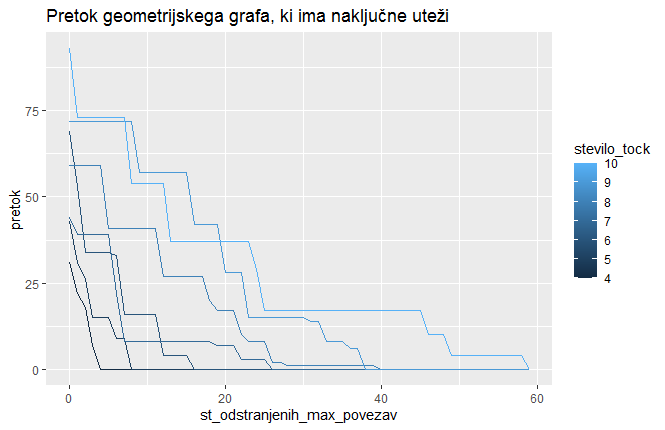
\includegraphics[scale=.5]{p9_1.PNG}}
\caption{Pretok pri geometrijskem grafu ($tip = 3$), ki mu odstranjujemo maksimalno utež na povezavi.}
\label{fig14}
\end{figure}  

$\rightarrow$ Geometrijski grafi, glede na spreminjanje razdalje r. V grafu so tiste povezave katera razdalja je manjša od r. Gledamo kako se spreminja pretok ko r teče od $0.1$ do $\sqrt{2}$, z razmikom $0.1$.  \\


$\ast$ Na grafu \ref{fig15} je prikazan geometrijski graf, ki ima za uteži kar razdaljo med točkami. Kot je ravidno je pri majhnem r-ju pretok v večini primerih enak 0, saj je takrat zelo malo povezav v grafu. Ko se r veča pa je seveda pretok večji. Največji pretok naj bi imel graf z desetimi točkami, najmanši pa z štirimi. Kot vidimo tukaj ni ravno tako, v grafu imamo veliko skokov, katero posledico bova opisala kasneje.
\begin{figure}[H]
\centerline{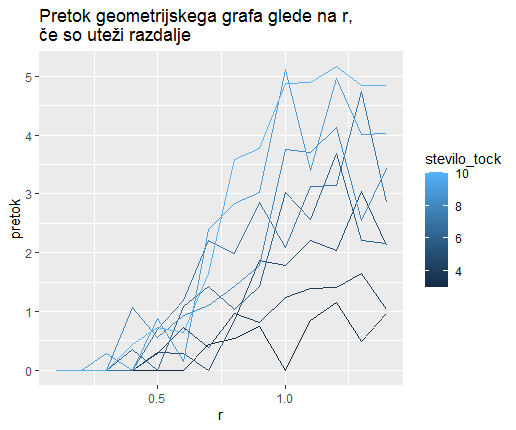
\includegraphics[scale=.6]{p10.PNG}}
\caption{Pretok pri geometrijskem grafu ($tip = 1$), kjer spreminjamo r.}
\label{fig15}
\end{figure} 

$\ast$ Na grafu \ref{fig15} je prikazan geometrijski graf, ki ima uteži inverz razdalj med točkami. Tukaj so skoki še bolj očitni, saj ima graf z naprimer 4 točkami pri $r = 0.3$ večji pretok, kot graf pri $r = 0.4.$ Vendar kljub temu lahko sklepamo, da se s povečevanje r-ja pretok veča. 
\begin{figure}[H]
\centerline{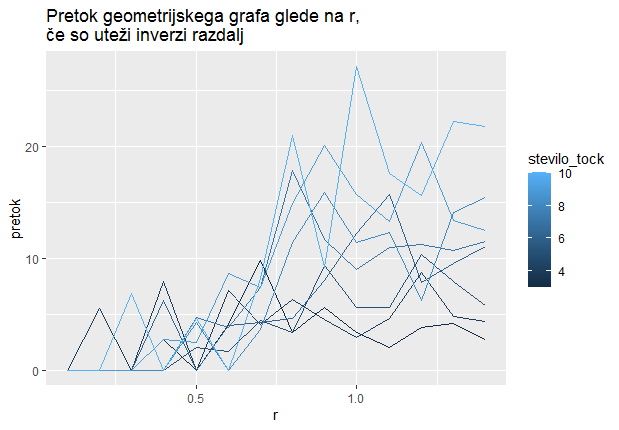
\includegraphics[scale=.6]{p11.PNG}}
\caption{Pretok pri geometrijskem grafu ($tip = 2$), kjer spreminjamo r.}
\label{fig15}
\end{figure} 


$\ast$  Na grafu \ref{fig16} je prikazan geometrijski graf, ki ima za uteži naključna cela števila do 10. Kot zgoraj je graf malo napačen, vendar je sklep isti. Graf z manj točkami imajo manjši pretok, kot grafi z več. Graf z isto številom toč ima pri manjšem r-ju majši pretok, kot pri velikem. 
\begin{figure}[H]
\centerline{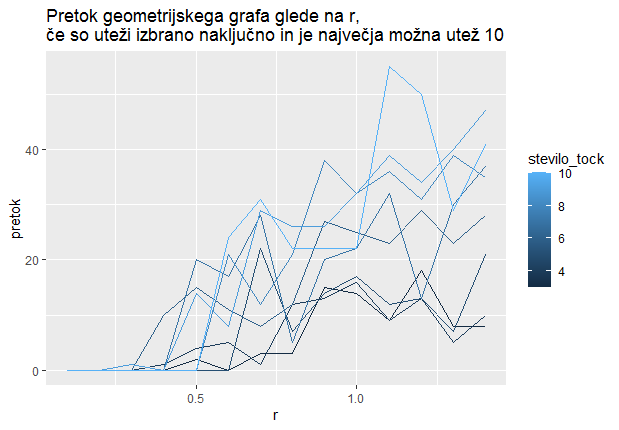
\includegraphics[scale=.6]{p12.PNG}}
\caption{Pretok pri geometrijskem grafu ($tip = 3$),  kjer spreminjamo r.}
\label{fig16}
\end{figure} 

Če povzamemo vse skupaj, lahko vidimo da neglede kaj odstranimo ali so to točke ali povezave je pretok manjši, kot pričakovano. Razlika je le v tem kako hitro pride do ničelnega pretoka, seveda je to odvisno tudi od podameznega grafa. Pri spreminjanje razdalje med točkami pa je pri večjem r večji pretok. \\


Naj omeniva še pomankljivost, ki sva jo opazila in je predvsem v grafih, kjer spreminjava r zelo očitna. Vemo da bi moral biti pretok pri grafu z 10 točkam, v večini primerih večji tok pretok pri grafu z manj točkami. Enako, če grafu odstranimo povezavo bo pretok enak oziroma manjši, kar pa pri nama ne drži nujno.  Kot opazimo pri najinih grafih se ponekod, grafi z manj točkami imajo večji pretok kot grafi z več točkami. Še najbolj očitno je to pri spreminjanju razdalje r. Kjer ima graf z večjim r manjši pretok, kot graf z majhnimr, kar pa ni logično. To je zato ker, sva narobe generirala podatke. Se pravi ko sva odstranila točko oziroma povezavo, sva graf ponovno zgenerirala seveda z manj točkami in povezavami vendar zopet naključno. Kar je pripeljalo do takih skokov v grafu. Bolj relavantno bi bilo gledat pretok enga grafa in temu odstranjevat točke oziroma povezave. Vendar kljub tej napaki lahko iz grafov vidimo kako se spreminja pretok ob spreminjanju različnih parametrov grafa. 

\subsection{Hitrost funkcij}

Kot opisano zgoraj, naju je zanimala tudi učinkovitost najine funkcije. Kot sva že takoj ugotovila, najina prva funkcija za pretok je neučinkovita.  Medtem ko je $\text{edmond\_karp}$ v primerjavi z vgrajeno funkcijo maxFlowFordFulkerson tudi bolj neučinkovit, kar je bilo tudi za pričakovati. V spodnji preglednici imava naveden čas v sekundah kako hitro je izračunal pretok pri različnem številu točk v grafu. Kot primerjava ima vgrajena funkcija 30  točkah hitrost $0.11$ sekunde. 
\begin{center}
\begin{tabular}{ |c|c|c|c| } 
\hline
$st\_tock$ & $edmonds\_karp$ & $maxFlowFordFulkerson$ \\
\hline
3 & 0.16 & 0 \\ 
4 & 0.19 & 0 \\ 
5 & 0.17 & 0 \\ 
6 & 0.20 & 0 \\ 
7 & 0.25 & 0 \\ 
8 & 0.36 & 0 \\ 
9 & 0.29 & 0 \\ 
10 & 0.33 & 0 \\ 
11 & 0.45 & 0 \\ 
\hline
\end{tabular}
\end{center}

\end{document}